\documentclass[10pt]{article}
\usepackage[margin=1.5cm]{geometry}

\usepackage{fancyhdr}
\pagestyle{fancy}
\date{\today}
\lhead{Ben McDonough}

\usepackage{amsmath}
\usepackage{amsthm}
\usepackage{amssymb}
\usepackage{dsfont}
\usepackage{physics}
\usepackage{svg}
\usepackage{soul}
\usepackage{hyperref}
\usepackage{simpler-wick}

\newcommand{\kb}{k_{\text{B}}}
\newcommand{\Ham}{\hat{\mathcal{H}}}
\newcommand{\vecop}[1]{\hat{\vec{#1}}}

\newtheorem*{defn}{Definition}
\newcommand{\Lec}[1]{Lecture: #1 \\ \\ \noindent}

\renewcommand{\grad}{\vec \nabla}
\newcommand{\smallspace}{\hspace{2cm}}

\setulcolor{red}

\begin{document}
\section{Review of single particle quantum mechanics and statistical mechanics of a quantum system}

\subsection{Wave Function}
Max Born interpretation: probability density of finding a particle at a point $\vec r$ is
$$
P(\vec r, t) = \left|\psi(\vec r, t)\right|^2
$$
\subsection{Single-particle Schr\"odinger equation.}

$$
i\hbar \pdv{\psi}{t} = \Ham \psi \ , \smallspace \Ham = \frac{\hat p^2}{2m} + V(\hat{\vec r})
$$

In coordinate representation: $\vec p = -i\hbar $; $\Ham = -\frac{\hbar^2}{2m}(\grad^2)+V(\vec r)$
\subsection{Linear superposition of waves}
If $\psi_a(\vec r, t)$, $\psi_b(\vec r, t)$ are solutions of SE, then $\psi_c =  a\psi_a + b\psi_b$ is also a solution.

\subsubsection{Stationary states, eigenstates}
$$
\psi_n(\vec r, t) = e^{-i\varepsilon_n t/\hbar}\varphi_n(\vec r) \ \Rightarrow \ \Ham \varphi_n(\vec r) = \varepsilon_n \varphi_n(\vec r)
$$
$$
\psi(\vec r, t) = \sum_n \alpha_n e^{-i\varepsilon_n t/\hbar} \varphi_n(\vec r)
$$

\subsection{Quantum Gibbs distribution}

\begin{figure}[h]
  \centering
  \begin{minipage}[b]{0.25\textwidth}
    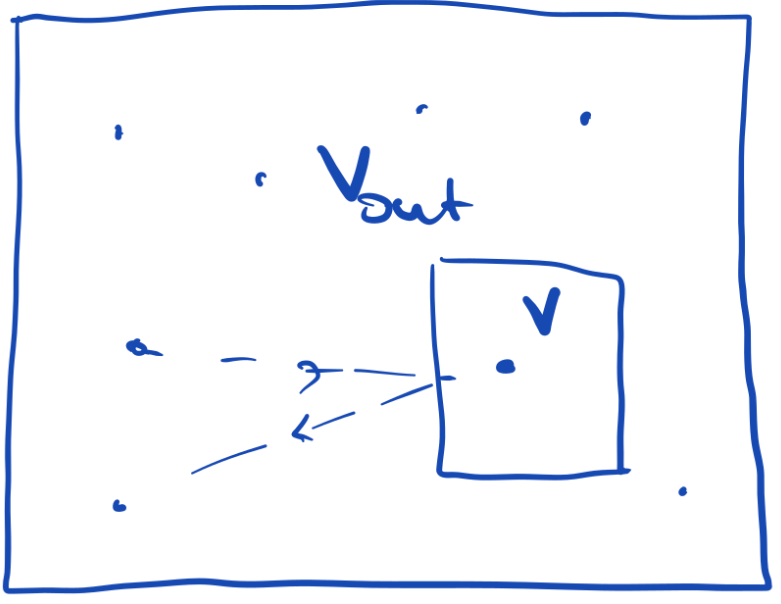
\includegraphics[width = \textwidth]{./figures/ss.png}
  \end{minipage}
  \begin{minipage}[b]{0.65\textwidth}
    \raggedright
    \begin{itemize}
        \item System wavefunction: $\psi(\vec r_1, \vec r_2, ..., \vec r_N)$
        \item Density matrix (coordinate representation:)
            $$\rho(\vec r_1, \vec r_1') \equiv \qty(\Pi_{i=2}^N)\psi^\ast(\vec r_1, \vec r_2, ..., \vec r_N)\psi(\vec r_1', \vec r_2', ..., \vec r_N')$$
        \item Probability density: $P(\vec r_1) = \rho(\vec r_1, \vec r_1)$
            \vspace{.4cm}
    \end{itemize}
  \end{minipage}
  \label{fig:densitymatrix}
\end{figure}
\noindent We may expand $\rho(\vec r, \vec r')$ in eigenfunctions $\psi_n(\vec r)$ of a single-particle Hamiltonian (describing an isolated particle)
$$
\rho(\vec r, \vec r') = \sum_{nm}w_{mn} \psi_n^\ast(\vec r) \psi_m(\vec r'); \smallspace \hat \rho = \underbrace{\sum_{nm}\ket{m}w_{mn}\bra{n}}_{\text{density matrix (Dirac notation)}}
$$
Quantum Gibbs distribution (equilibrium distribution): $\boxed{w_{mn} = \frac{1}{Z}e^{-\beta\varepsilon_n}\delta_{mn}}$, where $\beta = 1/\kb T$ (we will mostly stick to $\kb \to 1$)\\ \\
Quantum Gibbs distribution, statistical operator:
$$
\hat \rho_G = \frac{1}{Z}\sum_n \ket{n} e^{-\beta \varepsilon_n}\bra{n} = \frac{1}{Z}e^{-\beta \Ham}
$$
Partition function: $Z = \sum_{n}e^{\beta \varepsilon_n}$ (so that $\sum_n w_{nn} = 1$.) 
$$
Z = \sum_{n} e^{-\beta \varepsilon_n} = \sum_n \bra{n}e^{-\beta \Ham}\ket{n} = \Tr{e^{-\beta \Ham}}
$$

\hl{The traditional point of view} at microcanonical (fixed energy) and thermal (Gibbs) distributions is based on the motion of \hl{statistical ensemble}, see Huang, \hl{Stat. Mech. Ch. 8} and also employs the notion of ergodicity in evolution of a classical system. \\ \\
\noindent A modern point of view is based on the \hl{eigenstate thermalization hypothesis (ETH)}, see Mark Srednicki \href{https://arxiv.org/abs/cond-mat/9403051}{Chaos and Quantum Thermalization}, Phys. Rev. E, 50, 888(1994)

\subsection{Classical limit in statistical mechanics:}
$$
Z_{cl} = \frac{1}{(2\pi \hbar)^d}\int d^d\vec p \int d^d \vec x e^{-\beta \mathcal{H}(\vec p, \vec x)} \smallspace \text{v.s.} \smallspace Z = \Tr{e^{-\beta \Ham}}
$$
Example: \textit{1D Harmonic Oscillator:} $\Ham = \frac{\hat p^2}{2m} + \frac{m\omega_0^2}{2}x^2$ (1D)
\begin{align*}
    \varepsilon &= (n+\frac{1}{2r \omega_0}) & Z &= \sum_{n=0}^\infty e^{-\beta \hbar \omega_0(n+ \frac{1}{2})} = \frac{e^{-\beta\hbar \omega_0/2}}{1-e^{-\beta\hbar \omega}} = \frac{1}{2\sinh(\beta \hbar \omega_0 / 2)}
\end{align*}
Classical limit: $\beta \hbar \omega_0 \ll 1 \ \Rightarrow Z \simeq \frac{1}{\beta\hbar\omega_0}$
$$
Z_{cl} = \frac{1}{2\pi \hbar}\int_{-\infty}^\infty dp \int_{-\infty}^\infty dx e^{-\beta\left(\frac{p^2}{2m}+\frac{m\omega_0^2}{2}x^2\right)} = \frac{1}{2\pi \hbar} \int_{-\infty}^\infty dp e^{-\frac{\beta p^2}{2m}} \int_{-\infty}^\infty dx e^{-\frac{\beta m\omega_0^2}{2}x^2} = \frac{1}{\beta\hbar \omega_0}
$$
$\frac{1}{2\pi \hbar}$ in $Z_{cl}$ gives the correct state counting $(\Delta p \Delta x = 2\pi \hbar$ per state).

\subsection{Free energy}
    $$
F = -T\ln Z
    $$
    Classical description of harmonic oscillator:
    $$
F_{cl} = -T\ln Z = -T \ln (\frac{T}{\hbar \omega_0}) \smallspace S = -\pdv{F}{T} \ \ \text{(entropy, as defined in thermodynamics)}
    $$
    $$
S_{cl} = -\pdv{F_{cl}}{T} \underbrace{=}_{\text{for oscillator}} 1 + \ln(\frac{T}{\hbar\omega_0}) \smallspace \text{\textit{problem at $T = 0$!}}
    $$
full quantum result for oscillator (with $Z = \sum_n e^{-\beta \varepsilon_n}$):
\begin{align*}
    F &= \frac{1}{2}\hbar \omega_0 + T \ln(1-e^{\beta \hbar \omega_0}) \\
    S &= -\ln(1-e^{-\hbar \omega_0 / T}) + \frac{\hbar \omega/T}{e^{\frac{\hbar \omega_0}{T}}-1} \\
    S &\propto \frac{\hbar \omega_0}{T}e^{-\hbar \omega_0/T} \ \text{at} \ T \to 0
\end{align*}
Entropy (the density matrix definition):
$$
S = \ln [\text{number of available states}] = -\sum_n w_n \ln w_n; \ \ \text{$w_n$ is the probability of state $n$ occupation}
$$
Yields the thermodynamic definition of $S$ for Gibbs distribution $\omega_n$.

\subsection{Expectation values}
$\hat O$: operator of a (measurable) quantity. \ul{Expectation value} for a given \textcolor{red}{pure} state: $\bra{\psi}\hat O \ket{\psi}$, e.i., average of $\hat O$ over a state $\ket{\psi}$.\\ \\
\noindent In the eigenstates of a Hamiltonian representation: $\psi = \sum_n \alpha_n \ket{n}$:
$$
\bra{\psi}\hat O \ket{\psi} = \sum_{mn} \alpha_m^\ast \alpha_n \bra{m}\hat O \ket{n} \equiv \sum_{mn} \alpha_m^\ast \alpha_n O_{mn}
$$
$$
\bra{m}\hat O \ket{n} = O_{mn} = \text{matrix element of $\hat O$ in the eigenstates basis}
$$
Time-averaged expectation value for a \textcolor{red}{pure} state:
$$
\psi = \sum_n \colorbox{yellow}{$\alpha_n$} \ket{n} \ \Rightarrow \psi(t) = \sum_n \alpha_n e^{-\varepsilon_n t/\hbar}\ket{n}
$$
$$
\colorbox{yellow}{$\bra{\psi(t)}\hat O \ket{\psi(t)}$} = \sum_{nm} \colorbox{yellow}{$\alpha_m^\ast \alpha_n e^{i\frac{\varepsilon_m - \varepsilon_n}{\hbar}t}$} O_{mn}
$$
time-averages value: $\overline A \equiv \lim_{t_0 \to \infty} \int_0^{t_0} dt A(t)$
$$
\overline{\bra{\psi(t)}\hat O \ket{\psi(t)}} = \sum_{nm}\alpha_m^\ast \alpha_n \overline{e^{i\frac{\varepsilon_m - \varepsilon_n}{\hbar}t}}O_{mn} = \sum_n |\alpha_n|^2 O_{nn}
$$
In general, depends on the initial state (\hl{via $\alpha_n$}). ETH states that for a \hl{large} (infinite in the limit) system and a \hl{local quantity $\hat O$}, $|\alpha_n|^2$ depend only on the state's energy $E_n$. \\ \\

\textcolor{magenta}{\ul{Expectation value} of $\hat O$ for a \ul{mixed state} described by a density matrix}\\ \\

Return for a minute to the definition of expectation values for a one-particle system and write it out using the real-space coordinate representation:
$$
\bra{\psi}\hat O \ket{\psi} = \int d\vec r \psi^\ast(\vec r) \hat O(\vec r, \vec p)\psi(\vec r)
$$
Now suppose we have a may-particle system in a purse state, $\psi(\vec r_1, \vec r_2, ..., \vec r_N)$, but still are interested in the expectation value of an observable associated with one specific particle, namely particle 1: $\hat O(\vec r_1, \hat{\vec p}_1)$.  \\
We will start now from the already introduced definition of the expectation value, $\bra{\psi}\hat O \ket{\psi}$, and see how to abbreviate it using the notion of the density matrix $\rho(\vec r, \vec r'),$ defined earlier
$$
\rho(\vec r_1', \vec r_1) \equiv \qty(\prod_{i=2}^N \int d\vec r_i)\psi^\ast(\vec r_1', \vec r_2, .., \vec r_n)\psi(\vec r_1, \vec r_2, ..., \vec r_N
$$
Indeed,
\begin{align*}
    \bra{\Psi}\hat O \ket{\Psi} &= \int d \vec r_1 \int \prod_{i=2}^N d \vec r_i \psi^\ast(\vec r_1, \vec r_2, ..., \vec r_N)\hat O(\vec r_1, \vecop p_1)\psi(\vec r_1, \vec r_2, ..., \vec r_N)\\
                                &= \int d \vec r_1 \int \prod_{i=2}^N d \vec r_i \psi^\ast(\vec r_1, \vec r_2, ..., \vec r_N)\hat O(\vec r_1, \vecop p_1)\int d\vec r'_1\delta(\vec r_1-\vec r_1')\psi(\vec r_1', \vec r_2, ..., \vec r_N)\\
                                &= \int d \vec r_1' \int d \vec r_1 \int \prod_{i=2}^N d \vec r_i \psi^\ast(\vec r_1, \vec r_2, ..., \vec r_N)\hat O(\vec r_1,\vecop p_1)\delta(\vec r_1-\vec r_1')\psi(\vec r_1', \vec r_2, ..., \vec r_N)\\
                                &= \int d\vec r_1' \int d\vec r_1 \rho(\vec r_1, \vec r_1')\hat O(\vec r_1, \vecop{p}_1)\delta(\vec r_1-\vec r_1')
\end{align*}
Now we can use a suitable complete basis of single-particle wave functions:
$$
\rho(\vec r, \vec r')  = \sum_{nm} w_{nm}\psi_n^\ast(\vec r) \psi_m(\vec r'); \ \hat \rho = \sum_{nm} \ket{m} w_{mn} \bra{n}
$$
Substitution of $\rho(\vec r, \vec r')$ in this form to the last line above yields
$$
\bra{\Psi}\hat O \ket{\Psi} = \int d \vec r_1' \int d r_1 \sum_{nm} w_{mn} \psi^\ast_n(\vec r_1) \psi_m(\vec r') \hat O (\vec r_1, \vecop p_1) \delta(\vec r_1 - \vec r_1')
$$
\setulcolor{black}
Noting that $\vecop p_1$ acts on $\vec r_1$ but \ul{not} on $\vec r_1'$, we may re-write
\begin{align*}
    \bra{\Psi}\hat O \ket{\Psi} &= \int d\vec r_1 \sum_{nm} w_{mn} \psi_n^\ast(\vec r_1)\hat O(\vec r_1, \vecop p_1) \int d\vec r_1' \delta(\vec r_1-\vec r_1') \psi_m(\vec r_1')\\
                                &= \sum_{nm}w_{mn}\underbrace{\int d\vec r_1 \psi^\ast _n(\vec r_1) \hat O(\vec r_1, \vecop p_1) \psi_m(\vec r_1)}_{O_{mn}} = \sum_{nm}\omega_{mn}O_{nm}
\end{align*}
$$
\boxed{\langle \langle \hat O \rangle \rangle = \sum_{nm} w_{mn} O_{nm} = \sum_{m}\sum_n \omega_{mn}O_{nm} = \Tr{\hat \rho \hat O}}
$$
Unless the function $\psi(\vec r_1, \vec r_2, ..., \vec r_N)$ is factorizable, $\psi(\vec r_1, \vec r_2, ..., \vec r_N) = \psi(\vec r_1)\cdot \psi(\vec r_2, ...., \vec r_N)$, the density matrix $\hat \rho$ corresponds to a mixed state of particle 1. The density matrix definition of the expectation value of $\hat O(-\vec r_1, \vecop p_1)$ is agnostic wrt states of other particles.\\ \\
\noindent Within ETH, a \hl{thermal ensemble average of a local quantity can be obtained as an expectation value over a pure state} with energy $\propto T \cdot N$ of a large system ($N \gg 1$).
\begin{figure}[hbt!]
    \centering
    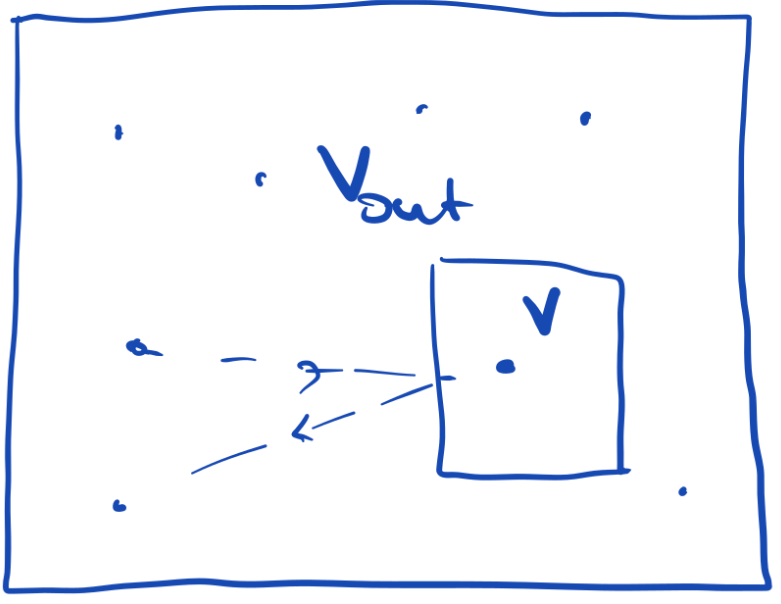
\includegraphics[width = .25\textwidth]{./figures/ss.png}
    \caption{We may consider a system with particle 1 confined to volume $V$, while other $N-1$ particles reside in volume $V_{out}$.}
\end{figure}
Assuming that particle 1 interacts with the other particles, but that interaction is weak compared to single-particle energies $\varepsilon_m$ and \hl{assuming the ETH is valid}, we may use $w_{mn} = \frac{1}{Z} e^{-\beta \varepsilon_m\delta_{mn}}$ (Gibbs distribution) to evaluate $\langle \langle \hat O \rangle \rangle$:
$$
\colorbox{yellow}{$\langle \langle \hat O \rangle \rangle$} = \frac{1}{Z}\sum_{m}e^{-\beta \varepsilon_m}O_m = \colorbox{yellow}{$\frac{1}{Z}\Tr{e^{-\beta \Ham}\hat O}$}
$$
\hl{In the conventional language, this is operator $\hat O$ averaged over the Gibbs (i.e. thermal) ensemble,}
$$
\hat \rho_G = \frac{1}{Z}\sum_m \ket{m}e^{-\beta \varepsilon_m}\bra{m}
$$
\section{Identical Particles}
\subsection{Many-body wave function and particle density}
$$
P(\vec R, t) = \qty|\psi(\vec R, t)|^2 \ ; \smallspace P(\vec R, t) = \int d\vec r \psi^\ast(\vec r, t) \delta(\vec R - \vec r) \psi(\vec r, t)
$$
$$
\hat n(\vec R) = \delta(\vec R - \vecop r)
$$
Joint probability density with finding particle 1 at $\vec r_1$, particle 2 at point $\vec r_2, ...,$ particle $N$ at point $\vec r_N$:
$$
P(\vec r_1, \vec r_2, ..., \vec r_N) = \qty|\psi(\vec r_1, \vec r_2, ..., \vec r_N)|^2
$$
Particle density operator: $\hat n(\vec R) = \sum_{j=1}^N \delta(\vec R - \vecop r_j)$ \\ \\
\noindent Expectation value of $\hat n(\vec R):$
$$
\hat n(\vec R) = \int d\vec r_1 d\vec r_2 ... d\vec r_N \psi^\ast(\vec r_1, \vec r_2, \hdots, \vec r_N) \hat n(\vec R) \psi(\vec r_1, \vec r_2, \hdots, \vec r_N)  =  \int d\vec r_1 d\vec r_2 ... d\vec r_N\qty|\psi(\vec r_1, \hdots, \vec r_N)|^2\sum_{j=1}^N\delta(\vec R - \vec r_j)
$$
Consider identical particles: $P(\vec r_1, \hdots, \vec r_N)$ is invariant with respect to coordinates permutation:
$$
\qty|\psi(\vec r_1, \hdots, \vec r_i, \hdots,\vec r_j, \hdots, \vec r_N)|^2 = \qty|\psi(\vec r_1, \hdots, \vec r_j, \hdots, \vec r_i, \hdots, \vec r_N)|^2
$$
\subsection{Operator of permutation}
$$
\hat P_{ij}\psi(\vec r_1, \hdots, \vec r_i, \hdots, \vec r_j, \hdots, \vec r_N) = \psi(\vec r_1, \hdots, \vec r_j, \hdots, \vec r_i, \hdots, \vec r_N)
$$
$\qty|\psi(\vec r_1, \hdots, \vec r_N)|^2$ is invariant with respect to $\hat P_{ij}$. For a system of identical particles, operators of observable $\colorbox{yellow}{Classical limit!} Z_N = \frac{1}{N!}(Z_1)^N$. Note that the full QM result, $Z = \Tr{e^{-\beta \Ham}}$, differentiates between statistics, as the complete bases functions are different between Bose and Fermi statistics. \textcolor{purple}{Huang, Stat. Mech., 2${}^\text{nd}$ edition, Sec. 6.6 and 9.2}
\subsection{Exchange Energy}
Consider the example of 2 particles $\Ham_0 = \hat h(\vec p_1, \vec r_1) + \hat h(\vec p_2, \vec r_2)$, with $\hat h = \frac{p^2}{2M} + U(\vec r)$. The normalized eigenfunctions are $\hat h \psi_n = \varepsilon \psi_n$, $n = 0,1,\hdots$, and $\Vert \psi_n \Vert = 1$. 
$$
\psi_{m,n}^\pm (\vec r_1, \vec r_2) = \frac{1}{\sqrt{2}}\qty[\psi_m(\vec r_1)\psi_n(\vec r_2)\pm \psi_m(\vec r_2)\psi_n(\vec r_1)]
$$
$$
\braket{\psi^\pm_{m,n}}{\psi^\pm_{mn}} = 1 \ \text{if} \ \Vert \psi_n \Vert = 1, \ \text{and} \ m \neq n
$$
$m = n$:
\begin{itemize}
    \item[]Fermions: $\psi_{m,m}^- = 0$ (Pauli principle) 
    \item[]Bosons: $\psi_{m,m}^+ = \sqrt{2}\psi_m(\vec r_1)\psi_m(\vec r_2);$ to normalize: $\psi_m = \frac{1}{\sqrt{2!}}\psi^+_{m,m}$
\end{itemize}
%Note: maybe add the argument about constructing a projector onto the symmetrized/antisymmetrized subspace?
Ground state energy for 2 particles::
\begin{itemize}
    \item[]Fermions: $\psi_g = \psi^-_{0,1}; \ \varepsilon_g = \varepsilon_0 + \varepsilon_1$
    \item[]Bosons: $\psi_g = \frac{1}{\sqrt{2!}}\psi_{0,0}^+ = \psi_0(\vec r_1)\psi_0(\vec r_2); \ \varepsilon_g = 2\varepsilon_0$
\end{itemize}
\begin{align*}
    \mathcal H_0 \psi_{m,n} &= (\varepsilon_n + \varepsilon_m)\psi_{m,n} \ m\neq n; & \varepsilon_{m,n}^{(0)} &= \varepsilon_{m} + \varepsilon_{n} \\
    \mathcal H_0 \psi_{m,m} = 2\varepsilon_m\psi_{m,m}; & \varepsilon{m,m}^{(0)} = 2\varepsilon_m \ \text{(bosons)}
\end{align*}
Introduce a weak interaction $V(\vec r_1 - \vec r_2)$ between articles. We want to find correction to $\varepsilon_m,n^{(0)}$ due to interaction.\\
1${}^{st}$ order correction $\delta \varepsilon$ to $\varepsilon_{m,n}^{(0)}$:
\begin{align*}
    \delta \varepsilon &= \bra{\psi_{m,n}^\pm}\hat V \ket{\psi_{m,n}^\pm}\\
                       &= \frac{1}{2} \int d\vec r_1 d\vec r_2 \qty|\psi_m(\vec r_1)\psi_n(\vec r_2) \pm \psi_m(\vec r_2)\psi_n(\vec r_1)|^2V(\vec r_1- \vec r_2)\\
                                                    &= \frac{1}{2}\int d\vec r_1 d\vec r_2(\psi_m(\vec r_1)\psi_n(\vec r_2) \pm \psi_m(\vec r_2)\psi_n(\vec r_1))^\ast (\psi_m(\vec r_1)\psi_n(\vec r_2) \pm \psi_m(\vec r_2)\psi_n(\vec r_1))V(\vec r_1 - \vec r_2) \\
                                                    &= \frac{1}{2}\int d\vec r_1 d\vec r_2 \qty(\qty|\psi_m(\vec r_1)|^2 \qty|\psi_n(\vec r_2)|^2+\qty|\psi_m(\vec r_2)|^2\qty|\psi_n(\vec r_1)|^2)V(\vec r_1 - \vec r_2) \\
                &\smallspace\pm \frac{1}{2}\int d\vec r_1 d\vec r_2\left\{\psi_m^\ast(\vec r_1)\psi_n(\vec r_1) \psi_n^\ast(\vec r_2)\psi_m(\vec r_2) + \psi_m(\vec r_1)\psi_n^\ast(\vec r_1)\psi_n(\vec r_2) \psi_m^\ast (\vec r_2)\right\}V(\vec r_1 - \vec r_2)\\
                &= \int d\vec r_1 d\vec r_2 \overbrace{\qty|\psi_m(\vec r_1)|^2 \qty|\psi_n(\vec r_2)|^2 V(\vec r_1 - \vec r_2)}^{\text{\textcolor{red}{density-density interaction}}} \underbrace{\pm \int d\vec r_1 d\vec r_2 \Re\left\{(\psi_m^\ast(\vec r_1)\psi_n(\vec r_1))(\psi^\ast_n(\vec r_2)\psi_m(\vec r_2)\right\}V(\vec r_1 - \vec r_2)}_{\text{\textcolor{red}{exchange energy}}}
\end{align*}

\subsection{N-particle generalizations}
\subsubsection{Fermions}
$$
\hat P_{nm} \psi(\vec r_1, \vec r_2, \hdots, \vec r_n, \hdots, \vec r_m, \hdots, \vec r_N) = \hat P_{nm} \psi(\vec r_1, \vec r_2, \hdots, \vec r_m, \hdots, \vec r_n, \hdots, \vec r_N)
$$
Fermion wave function satisfies:
$$
\hat P_{nm} \psi(\vec r_1, \vec r_2, \hdots, \vec r_n, \hdots, \vec r_m, \hdots, \vec r_N) = 
(-1) \cdot \hat P_{nm} \psi(\vec r_1, \vec r_2, \hdots, \vec r_n, \hdots, \vec r_m, \hdots, \vec r_N)
$$
To construct a convenient basis for $N$ fermions, consider an orthonormal set of single-particle states $\psi_j(\vec r_i)$ and form an antisymmetric combination:
$$
\psi = \frac{1}{\sqrt{N!}}\hat A \psi_{j_1}(\vec r_1)\psi_{j_2}(\vec r_2)\hdots\psi_{j_N}(\vec r_N)
$$
with $\hat A$ being the antisymmetrization operator acting on $\{\vec r_i\}$. Introduce operator of permutation
$$
P\{1,2,3,\hdots,N\} = \{P_1, P_2, P_3, \hdots, P_N\} \smallspace P_k = P(k) \ \text{is an image of integer $k$}
$$
\begin{itemize}
    \item \textbf{Even permutation $P$}: involves an even number of pairwise permutations to achieve 
        $$
        \{P_1, P_2, P_3, \hdots, P_N\}; \ (-1)^P = 1
        $$
    \item \textbf{Odd permutation}  $P$: involves an odd number of pairwise permutations to achieve 
        $$
        \{P_1, P_2, P_3, \hdots, P_N\}; \ (-1)^P = -1
        $$
\end{itemize}
Example:
\begin{align*}
    &\{1,2,3\}\\
    &\{\wick{\c1 3,2,\c1 1}\} \ \text{odd} \\
    &\{\wick{\c1 2,\c1 3,1}\} \ \text{even}
\end{align*}
$$
\psi = \frac{1}{\sqrt{N!}}\hat A \psi_{j_1}(\vec r_1)\psi_{j_2}(\vec r_2)\hdots\psi_{j_N}(\vec r_N) = \frac{1}{\sqrt{N!}}\sum_{\{P\}}(-1)^{P}\psi_{j_1}(\vec r_{P_1})\psi_{j_2}(\vec r_{P_2})\hdots\psi_{j_N}(\vec r_{P_N}) = \frac{1}{\sqrt{N!}}\det M
$$
Matrix elements of $M$: $M_{ij} = \psi_i(\vec r_j)$
$$
\psi = \frac{1}{\sqrt{N!}}\mqty|\psi_{j_1}(\vec r_1) & \hdots & \psi_{j_1}(\vec r_N) \\ \vdots & & \vdots \\ \psi_{j_N}(\vec r_1) & \hdots & \psi_{j_N}(\vec r_N)| \smallspace \text{Slater determinant}
$$
We may define $\psi$ by allowing $P$ to act on $\{j_l\}$ instead of $\{\vec r_i\}$:
$$
\psi = \frac{1}{\sqrt{N!}}\hat A \psi_{j_1}(\vec r_1)\psi_{j_2}(\vec r_2)\hdots \psi_{j_N}(\vec r_N) = \frac{1}{\sqrt{N!}}\sum_{\{P\}}(-1)^P \psi_{j_{P_1}}(\vec r_1)\psi_{j_{P_2}}(\vec r_2)\hdots \psi_{j_{P_N}}(\vec r_N) = \frac{1}{\sqrt{N!}}\det M^\top
$$
Matrix elements of $M^\top$: $M^\top_{ij} = \psi_j(\vec r_i)$
$$
\psi = \frac{1}{\sqrt{N!}}\mqty|\psi_{j_1}(\vec r_1) & \hdots & \psi_{j_N}(\vec r_1) \\ \vdots & & \vdots \\ \psi_{j_1}(\vec r_N) & \hdots & \psi_{j_N}(\vec r_N)|
$$
The introduced many-body function is normalized:
$$
\braket{\psi}{\psi} = \frac{1}{N!}\sum_{\{P\}}\sum_{\{P'\}}(-1)^{P+P'}\prod_{k=1}^N\braket{\psi_{j_{P_k}}}{\psi_{j_{P'_k}}} = \frac{1}{N!}\sum_{\{P\}}\sum_{\{P'\}}(-1)^{P+P'}\delta_{PP'} = \frac{1}{N!}\sum_{\{P\}}\sum_{\{P'\}}\delta_{PP'} = \frac{1}{N!}\sum_{\{P\}}1 = 1
$$
Consider a free-fermion system (no interactions) 
$$
\mathcal H = \sum_j h(\hat p_j, \hat r_j) \ \text{(symmetric in $(i,j)$ for all $(i,j)$}
$$
Pick $\psi_i(\vec r_j)$ in $\psi$ as eigenfunctions of $h(\hat p_j, \hat r_j)$. Suppose $\psi$ is constructed out of states $j_1, j_2, \hdots, j_N$. The eigenvalue of energy for $\psi$ is $E = \sum_{k=1}^N \varepsilon_{j_k}$\\
Introduce occupation numbers of single-particle states $n_k$\\
(fermions: $n_k = 0$ or $1$ depending on wither $j_k$ is present or absent in $\sum \hdots,$ respectively). We re-write
$$
\colorbox{yellow}{$E = \sum_{k=1}^\infty n_k \varepsilon_k, \ \sum_{k=1}^\infty n_k = N$}
$$

\subsubsection{Bosons}
$$
\psi \propto \sum_{\{\colorbox{yellow}{$P$}\}} \psi_{P_1}(\vec r_1)\hdots \psi_{P_N}(\vec r_N)
$$
We should symmetrize with respect to \hl{different one-particle states.} Introduce here too the occupation number $n_i$ of state $i$ (it is the number of coinciding indices in the above $\psi$)\\
The properly normalized function:
$$
\psi = \sqrt{\frac{n_1!n_2!...}{N!}} \sum_{\{P\}} \psi_{P_1}(\vec r_1)\hdots \psi_{P_N}(\vec r_N)
$$
$\{P\}$: all permutations of \hl{different} indices. The number of indices $P_1, \hdots, P_N$ is $\leq N$. Free-boson system: $E = \sum_{i=1}^\infty n_i \varepsilon_i; \ N = \sum_{i=1}^\infty n_i$ ($n_i$ may take values $0,1,\hdots$.)\\ \\
\textcolor{magenta}{More: Landau and Lifschitz v. 3, \textsection (you may like also \textsection 62, 63) + Negele-Orland, Sec. 1.2 and 1.3}
\section{Second Quantization}
1.26
\subsection{Boson Statistics}
\subsection{Fermions}
\subsection{Field Operators}
\subsection{Change of the one-particle basis in second quantization}
\subsection{Momentum representation of field operators}
\subsection{Time evolution of observables, equations of motion}
\section{Free fermions}
2.16
\subsection{Two point correlation  function of density in an ideal Fermi gas}
\subsection{Wick's theorem}
\subsection{Elementary theory of photoelectric effect and the fermion spectral function}
2.21\\
\begin{defn}[Spectral Function]
We consider an incident photon of momentum $\vec q$. The spectral function for a hole is defined
$$
A_h(\vec p, \omega) = \frac{1}{\pi}\Re \int_{-\infty}^0 dt e^{i\omega t + 0.t} \int d\vec r e^{-i\vec p \cdot \vec r} \bra{G} \psi^\dagger(0,0)\psi(\vec r, t)\ket{G}
$$
In terms of the probability amplitude for a hole to propagate from a point $\vec r$ at time $t$ to $0$ at time $0$ $\bra G \psi^\dagger(0,0) \psi(\vec r, t)\ket{G}$. Then the frequency of transition from an incident photon of momentum $\vec q$ to a scattered electron of momentum $\ket k$ is
$$
\omega_{\vec q, \vec k} = \frac{2\pi}{\hbar^2}|\lambda|^2 \int d\omega\delta(\omega + (\omega_{\vec q}-\frac{\hbar^2k^2}{2m}))\int d\vec p \delta(\vec p +\omega_{\vec q}-\vec k)) A_h(\vec p, \omega))
$$
\end{defn}
The spectral function for noninteracting fermions is
$$
A_h(\vec p, \omega)) = \theta(\varepsilon_F - \varepsilon(\vec p))\delta(\omega-\frac{\varepsilon(\vec p)}{\hbar}))
$$
The spectral function for a particle can be similarly constructed:
$$
A_p(\vec p, \omega) = \sum_n\qty|\bra{n}a_{\vec p}^\dagger \ket{G}|^2 \delta(\omega + \frac{1}{\hbar}(E_g(N+1)-E_n(N)))
$$
\subsection{Notion of the Fermi Liquid}
\Lec{2.28}
We consider the effect of the momentum-conserving interaction Hamiltonian
$$
\hat V = \frac{1}{2}\sum_{\vec p \vec p \vec q}v(\vec q) a_{\vec p - \vec q}^\dagger a^\dagger_{\vec p' + \vec q}a_{\vec p'}a_{\vec q}
$$
On the lifetime of the single-particle state with energy (momentum) $\xi, \vec p$. For the general 3D case, we have $\frac{1}{\tau} \propto \xi^2$. For the Coulomb interaction specifically,
$$
\frac{1}{\tau(\xi)} \sim \frac{e^2}{\hbar v_F}\frac{\xi^2}{E_F}
$$
For weak interactions, we take $n_p(t) \approx |\bra{G} a_p(t)a_p^\dagger(0) \ket{G}|^2 = e^{-t/\tau(\chi_p)}$, which leads to the Fermi liquid spectral function (in units with $\hbar = 1$),
$$
A(\vec p , \omega) = \Im \frac{1}{\omega-\xi_{\vec p} - i/2\tau(\xi_{\vec p})}
$$

\section{Linear response, FDT, and the dynamic structure factor}
\subsection{General Linear Response (Kubo Formula)}
\begin{defn}[Kubo formula]
We consider an observable $\hat A$ and a perturbation $\hat V(t) = f(t)\hat B$. The change in the expectation of $\hat A$ is
$$
\langle \delta \hat A \rangle = \frac{1}{i\hbar} \int_{-\infty}^t dt' \langle [A^I(t), B^I(t')]\rangle_0f(t')e^{0.t'}
$$
For the case of a time-translation invariant system, this is written
$$
\langle \delta A \rangle  = \frac{1}{i\hbar}\int_{-\infty}^\infty dt' \Pi^{AB}_R(t-t')f(t')
$$
\end{defn}
\begin{defn}[Retarded response function]
$$
\Pi^{AB}_R(t) =-\frac{i}{\hbar} \theta(t)\langle [A^I(t), B^I]\rangle_0
$$
also called the retarded correlation function.
\end{defn}

\subsection{Fluctuation-Dissipation Theorem (FDT)}
The imaginary part of the response function fourier components for an operator $\hat A$ to a perturbation by $\hat A$ can be evaluated:
$$
\Im \Pi_R(\omega) = \frac{\pi}{\hbar}(e^{-\beta \hbar \omega}-1)\sum_{mn}\frac{e^{-\beta E_m}}{A}\qty|A_{mn}|^2 \delta(\omega+\omega_m-\omega)
$$
Then we define the symmetrized correlation function (not distinguishing between absorption and scattering)
$$
\langle A^2 \rangle_\omega \equiv \int_{-\infty}^\infty dt \frac{1}{2} \langle \hat A(0) \hat (t) + \hat A(t) \hat A(0) \rangle_0 e^{i\omega t - 0.|t|}
$$
Expanding, this can be re-written as
$$
\langle A^2 \rangle_{\omega} = \pi (1+e^{-\beta \hbar \omega})\sum_{mn} \frac{e^{-\beta E_m}}{Z}|A_{nm}|^2\delta(\omega + \omega_m - \omega_n)
$$
Which in terms of the response function evaluates to 
$$
\langle A^2 \rangle_\omega = -\coth(\frac{\hbar \omega}{2\kb T})\hbar \Im \Pi_R(\omega)
$$
using the fact that $\Im \Pi_R(\omega)$ is an odd function of frequency, we have
$$
\langle A^2 \rangle_{0} = -\hbar \int_0^\infty \frac{d\omega}{\pi}\coth(\frac{\hbar \omega}{2\kb T})\Im \Pi_R(\omega)
$$

\subsection{Absorption power}
Why care about the imaginary part of $\Pi_R(\omega)$? Consider a time-dependent perturbation to a time-independent Hamiltonian $\hat V = V_0 \cos(\omega t)\hat A$. Then the absorption power is the time-average of the derivative of the expected energy, which can be expressed
$$
W \equiv \overline{\dv{H}{t}}^t = -\frac{1}{2}\omega V_{0}^2 \Im \Pi_R(\omega)
$$

\subsection{Dynamic density structure factor (DSF)}
\begin{defn}[DSF]
Assuming a translationally invariant system, the density structure is defined as the fourier transform of $\langle n(\vec r_1, t) n(\vec r_2, 0) \rangle$, which determines the linear response of $\hat n(t, t)$ to a field coupled to particle density;
$$
S(\vec q, \omega) = \int_{\infty}^\infty dt d\vec r e^{i\omega t}e^{iq\vec r} \langle n(\vec r, t)n(0, 0)\rangle = \int_{-\infty}^\infty dt e^{i\omega t}\langle \hat n_{\vec q}n(t)\hat n_{-\vec q}(0)\rangle_0
$$
\end{defn}
Now, consider a perturbation of the form
$$
\hat V = -\int d\vec r' r(\vec r', t) \hat n(\vec r', t) e^{-i\omega t} + h.c. = -(\sum_{\vec q}v_{\vec q}\hat n_{-\vec q}e^{-i\omega t} + h.c.)
$$
Using the Kubo formula and FDT,
$$
S(\vec q, \omega) = -2\hbar \frac{\Im \Pi_R(\vec q, \omega)}{1-e^{-\beta \hbar \omega}}
$$
Note that $S(\vec q, \omega)$ characterizes the rate of absorption of incoming photons while $\Im \Pi_R(\vec q, \omega)$ characterizes the absorbed power.

\subsection{Free Fermion response fucntion}
3.30
$$
\Pi_R(\vec q, \omega^+) = -\frac{1}{\hbar}\frac{1}{L^3}\sum_{\vec k}\frac{n_{\vec k}-n_{\vec k _+ \vec q}}{\frac{\varepsilon_{\vec k + \vec q}}{\hbar}-\frac{\varepsilon_{\vec k}}{\hbar}-(\omega + i\delta)}
$$
$$
\Im \Pi_R(\vec q, \omega) = -\pi \int \frac{d^k}{(2\pi)^d}(n_{\vec k}-n_{\vec k + \vec q})\delta(\varepsilon_{\vec k + \vec q} - \varepsilon_{\vec k}-\hbar \omega)
$$
The above is only nonzero for the region $k_F \geq \frac{m^\ast}{\hbar^2q}\qty|\hbar \omega - \frac{\hbar^2q^2}{2m}|$. (check why this is!)\\
A static potential does not lead to dissipation because $\Im \Pi_R(\vec q, \omega) \to 0$ as $\omega \to 0$.
Limits:
fig
\begin{figure}[ht]
    \centering
    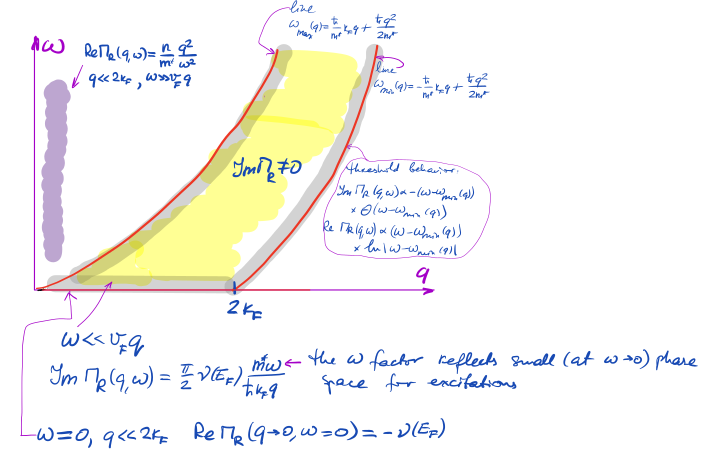
\includegraphics[scale=.4]{./figures/fig.png}
    \caption{Free fermion response in different limits}
    \label{fig:fig}
\end{figure}

\section{Random phase approximation}
4.04
Consider weakly interacting Fermions and a long-ranged potential produced by an external charge $v_{\vec q} = V_q n_q^{ext}$. The response function in RPA is
$$
\Pi^{RPA}(\vec q, \omega) = \frac{\Pi_0}{1-\Pi_0v_{\vec q}}
$$
where $\Pi_0$ is the response function of noninteracting fermions. This approximation is only valid for small $q$. \\
\subsection{Static limit, screening in RPA approximation}
Introduce the screened potential
$$
\delta n(\vec q, \omega) = \Pi(\vec q, \omega)v_{ext}(\vec q, \omega) = \Pi_0(\vec q, \omega)v_{sc}(\vec q, \omega)
$$
The dialectric function is defined as
$$
\frac{1}{\varepsilon(\vec q, \omega)}  = \frac{1}{1-\Pi_0(\vec q, \omega)} = 1+\Pi^{RPA}(\vec q, \omega)V_{\vec q}
$$
Plugging in the coulomb potential, we find
$$
V_{sc}(q) = \frac{4\pi e^2}{q^2+r_{TF}^{-2}}
$$
where $r_{TF} = (4\pi e^2 \nu_0)^{-\frac{1}{2}}$ is the Thomas-Fermi radius. 
\subsection{Plasma Oscillations}
\section{Mean field theory}
4.11
\subsection{Variational method}
Apply variational method to a trial free energy
$$
\Omega_{trial} = \Omega_0 + \langle H-H_0\rangle
$$
With $H = T +V$, $T = \sum_k(\varepsilon(\vec k)-\mu)c_{\vec k}^\dagger c_{\vec k}$ and $V = \frac{1}{2}\sum_{\vec k \vec p \vec q} v_(q) c_{\vec k + \vec q}^\dagger c_{\vec p - \vec q}^\dagger c_{\vec p}c_{\vec k}$, the self-consistency equation is 
$$
\Sigma(\vec k) = v(0) \sum_{\vec p}n_F(\varepsilon(\vec p) + \Sigma(\vec p)-\mu) \pm^B_F \sum_{\vec q}v(\vec q) n_F(\varepsilon(\vec k + \vec q)+ \Sigma(\vec k + \vec q)-\mu)
$$
The first term is the Hartree term, and the second term is the Fock or exchange term.
\subsection{Self-consistent field theory (another formulation of MFT)}
Like the homework, replace every $c^\dagger c$ with $\langle N \rangle$.
\subsubsection{Fermi liquid theory in Hartree-Fock approximation}
Effective mass $m^\ast$ comes from self-energy:
$$
\frac{m}{m^\ast} \equiv 1+ \pdv{\Sigma(k)}{\varepsilon(k)}\Big|_{k = k_F}
$$`
This comes from the definition of the fermi velocity,
$$
v_F = \frac{1}{\hbar}\dv{\vec k}(\varepsilon(\vec k)+\Sigma(\vec k))
$$
The heat capacity of noninteracting fermions is
$$
c_0(T) = \frac{\pi^2}{6}\kb^2\nu_0(E_F)T
$$
The Jacobian is renormalized by the interaction:
$$
\qty|\pdv{\varepsilon}{\vec k}| \to \qty|\pdv{\vec k}\qty(\varepsilon(\vec k)+ \Sigma(\vec k))|
$$
\subsection{Time-Dependent Hartree approximation}

\section{Weakly-interacting Bose gas}
\subsection{Uniform gas, Bogoliubov theory}
4.25
\subsection{Non-uniform interacting Bose gas at $T=0$}
\section{Superconductivity, BCS model}
\subsection{Scatting in Cooper Channel}
\subsection{The model Hamiltonian for many-body system, mean field solution}
\subsection{Josephson effect}
\subsection{Quantum fluctuations of phase, qubits}
\section{Green functions at $T=0$}
\section{Perturbations Theory for Green functions}

\end{document}
